%!TEX root = ../Allnew-Workspace.tex

\mychapter{적분법}{}

\section{적분법 : 미분법을 역이용하기}
지금까지는 원함수 $f\left( x \right) $가 주어졌을 때 도함수 $f'\left( x \right) $를 구하는 방법을 배웠습니다. 그렇다면 미분법을 역으로 이용하여 함수 $f(x)$가 어떤 함수 $F(x)$의 도함수일 때, 즉 $f(x)=F'(x)$일 때, $F(x)$를 찾는 방법이 존재할 것입니다. 이와 같이 $F(x)$를 찾는 것을 `$f(x)$를 \term{적분}{}한다'고 하며, 그 계산 방법을 \term{적분법}{}이라 합니다. 

\subsection{원시함수와 원함수의 정의}
함수 $f(x)$가 주어져 있을 때, $F'(x)=f(x)$를 만족시키는 함수 $F(x)$를 `함수 $f(x)$의 \term{원시함수}{}'라 합니다. 미분법에서 $f'(x)$,  $f(x)$를 각각 도함수와 원함수로 불렀듯이, 적분법에서도 $F(x)$와 $f(x)$를 각각 원시함수와 \iterm{원함수}{}로 부르도록 하겠습니다. 

\section{부정적분}
\subsection{원시함수의 성질과 부정적분의 정의}
$f(x)$의 원시함수 $F(x)$에 대하여 상수함수 $y=c$의 도함수는 $0$이므로 $F(x)+c$의 도함수는 $f(x)$입니다. 따라서 $F(x)+c$도 상수 $c$의 값에 관계없이 $f(x)$의 원시함수입니다. 이와 같이 $f(x)$의 원시함수는 유일하지 않습니다. 이러한 원시함수의 성질(유일하지 않음)에 착안하여 만들어진 용어가 \term{부정적분}{}입니다.\mn{\textbf{계산의 결과가 유일하게 정해지지 않고 무수히 많은 적분}이라는 의미입니다.}{}

함수 $f(x)$의 두 원시함수 $F(x)$, $G(x)$에 대하여 $F'\left( x \right) = f\left( x \right) $, $G'\left( x \right) = f\left( x \right) $이므로 다음이 성립합니다.
\begin{align*} \left\{ G\left( x \right) - F\left( x \right) \right\}' = G'\left( x \right) - F'\left( x \right) = f\left( x \right) - f\left( x \right)  = 0 \end{align*}
그런데 도함수가 $0$인 함수는 상수함수이므로, 그 상수를 $C$라 하면 $G\left( x \right)  - F\left( x \right)  = C$입니다. 따라서 $G\left( x \right) = F\left( x \right) +C$가 성립합니다.

지금까지 살펴본 바에 따르면, $f(x)$의 원시함수 중 하나를 $F(x)$라 하면 $f(x)$의 모든 원시함수, 즉 부정적분은
\begin{align*} F(x)+C \quad(\text{$C$는 상수})\end{align*}
로 나타낼 수 있습니다. 이를 기호로 다음과 같이 나타내며, 적분법 과정에서 나타나는 상수 $C$를 \term{적분상수}{}라고 합니다.
\begin{align*} \int f\left( x \right)dx = F(x) + C \quad(\text{단, $C$는 상수}) \end{align*}
\clearpage
\subsection{부정적분의 성질}\term{부정적분의 성질}{0}
부정적분은 다음과 같은 성질이 있습니다.
\begin{enumerate}[label={\onum*}]
    \item $\int k f\left( x \right) dx = k\int_{}^{}f\left( x \right) dx$ (단, $k$는 $0$이 아닌 상수)
    \item $\int \left\{ f\left( x \right) + g\left( x \right) \right\}   dx = \int_{}^{}f\left( x \right) dx + \int_{}^{}g\left( x \right) dx$
    \item $\int \left\{ f\left( x \right) - g\left( x \right) \right\}   dx = \int_{}^{}f\left( x \right) dx - \int_{}^{}g\left( x \right) dx$
\end{enumerate}

\section{$x^n$의 부정적분}\term{여러 가지 함수의 부정적분}{0}
미분법에 의하여 $\left( \dfrac{1}{n+1}x^{n+1} \right)' =  x^{n}$이므로 $\int x^n dx = \dfrac{1}{n+1}x^{n+1}+C$입니다.
%\subsection{$x^\alpha$의 부정적분}
%$\alpha \ne -1$일 때, $\dfrac{1}{\alpha+1}x^{\alpha+1}$의 도함수는 $x^\alpha$이므로 $\int_{}^{} x^\alpha dx = \dfrac{1}{\alpha+1} x^{\alpha+1}+C$입니다. 한편 로그함수 $\ln\abs{x}$의 도함수는 $\dfrac{1}{x}$이므로 $\int \dfrac{1}{x}dx = \ln\abs{x}+ C$입니다. 이를 이용하면 다항함수, 유리함수, 간단한 무리함수의 부정적분을 구할 수 있습니다.

\section{부정적분은 정적분을 계산하기 위한 수단}
한 점에서의 접선의 기울기와 접선의 방정식 구하기, 함수의 증감성 분석하기, (함수의 볼록성 분석하기)\mn{`함수의 볼록'은 \cnm{미적분}을 선택한 수험생에게만 해당됩니다.}{} 등 목적이 뚜렷했던 미분과 달리, 적분의 목적은 현재까진 알 수 없었습니다.

이는 부정적분이 그 자체로 의미를 갖기보다는, 곧 배울 정적분의 계산 수단에 불과하기 때문입니다. 정적분에는 명확한 목적이 있으므로, 일단은 `부정적분에서 이러한 계산이 가능하다'는 것만 숙지해둡시다.
\clearpage 

\section{구간넓이}
\begin{center}
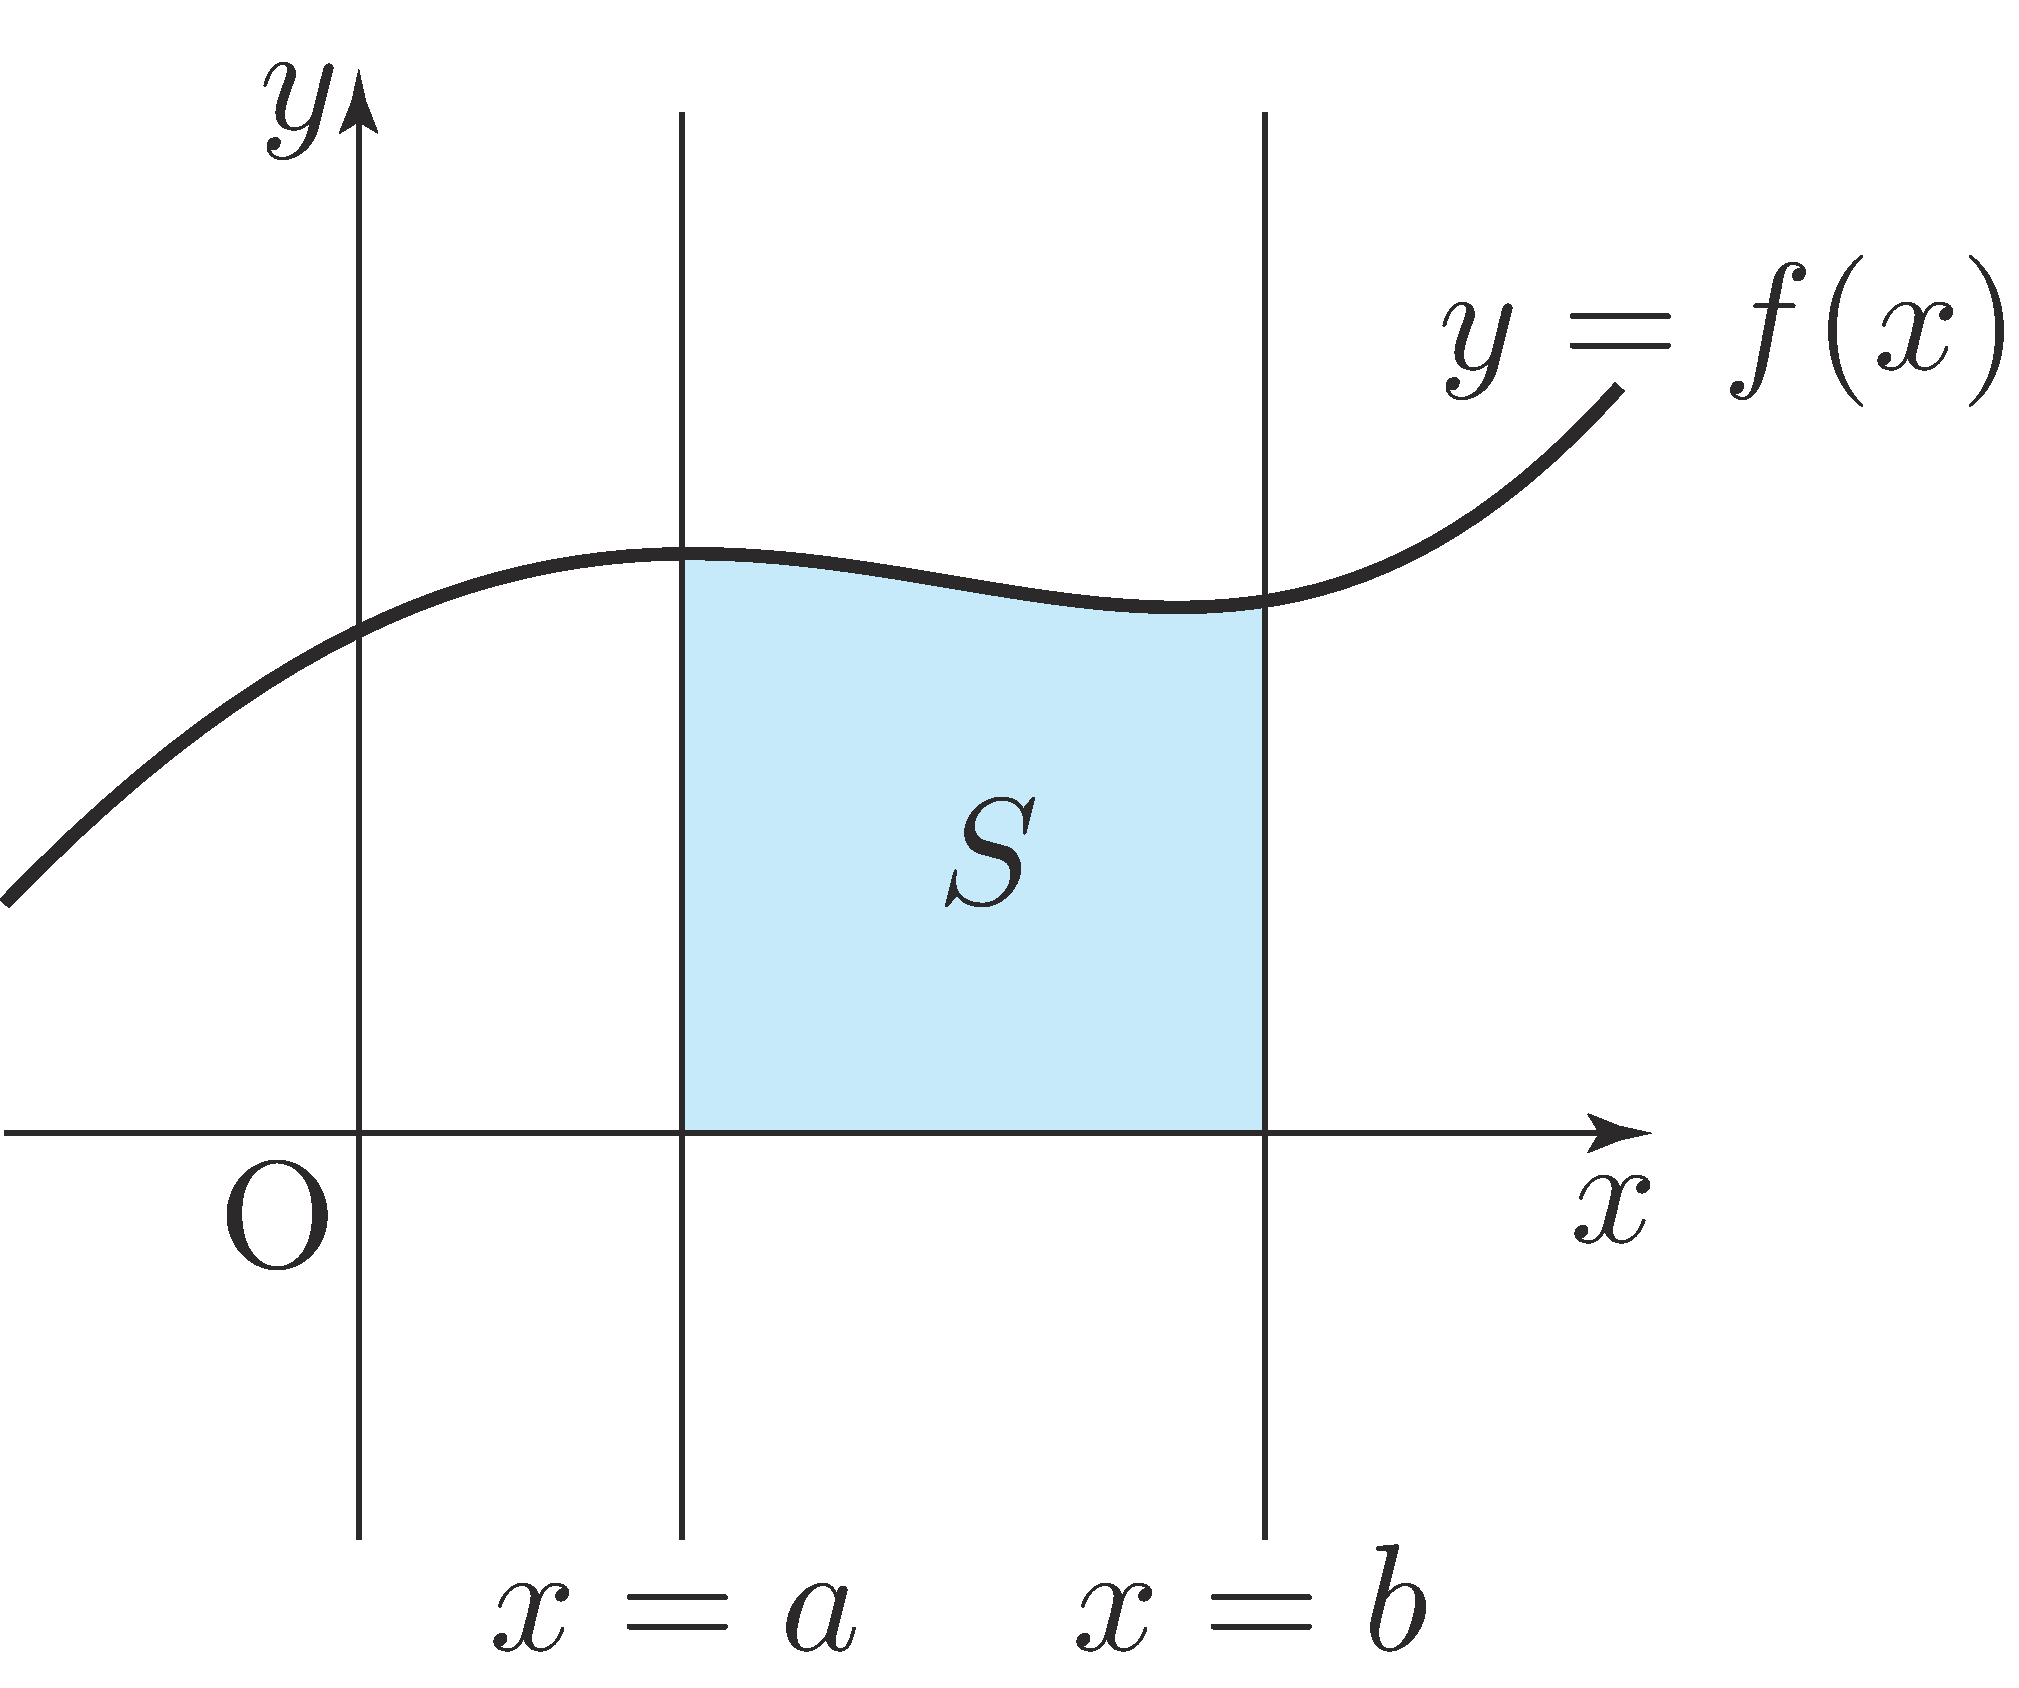
\includegraphics[scale=.125]{pic0/pic168.pdf}
  \end{center}  
  어떤 구간 $\CCI{a}{b}$에서 연속인 함수 $y=f(x)$에 대하여, 곡선 $y=f\left( x \right) $와 $x$축 및 두 직선 $x=a$, $x=b$로 둘러싸인 넓이를 $S$라 할 때, $S$를 `$\CCI{a}{b}$에서 $f\left( x \right) $의 \iterm{구간넓이}{}'라 부르기로 합시다.

\section{정적분}
정적분은 $\CCI{a}{b}$에서 $f\left( x \right) $의 구간넓이와 매우 밀접한 관계가 있는 수학적 도구입니다. 정적분을 이용하면 구간넓이를 구할 수 있습니다.

\subsection{정적분의 정의}

닫힌구간 $\CCI{a}{b}$에서 연속인 함수 $f\left( x \right) $의 한 부정적분을 $F\left( x \right) $라 할 때, $\int_{a}^{b} f(x) dx$를 \term{정적분}{}이라 하며, 다음과 같이 정의합니다.\mn{이는 본래 정적분의 정의가 아니라, 현 교육과정에서 억지로 정의했을 뿐입니다. 정적분의 진짜 정의는 따로 있으며, 본문에서 제시한 식은 \iterm{미적분의 기본 정리}{}입니다. 정적분의 진짜 정의는 무엇인지, 미적분의 기본정리는 어떻게 증명하는지, 그 의미는 무엇인지 궁금한 \cnm{미적분} 선택자는 \cnm{인투더 미적분}에서 이를 다루니 참고하기 바랍니다.}{}
\begin{align*}\int_{a}^{b}f\left( x \right)dx= \inti{F\left( x \right) }{a}{b} =F\left( b \right) - F\left( a \right)\end{align*}
    이때 $\int_{a}^{b} f(x) dx$는 `인티그럴 $a$에서 $b$까지 $f(x)dx$'라고 읽습니다. 또한 $a$를 \term{아래끝}{}, $b$를 \term{위끝}{}, $f(x)$를 \term{피적분함수}{}라 합니다. 한편 $dx$의 $d$ 뒤에 적힌 변수를 \term{적분변수}{}라 합니다.

\subsection{$a \ge b$일 때 정적분의 값}
$a=b$일 때, 즉 $\int_{a}^{b}f\left( x \right) dx= \int_{a}^{a}f\left( x \right) dx$일 때 $\int_{a}^{a}f\left( x \right) dx=0$입니다. $a>b$일 때, $\int_{a}^{b}f\left( x \right) dx = -\int_{b}^{a}f\left( x \right) dx$입니다.
\clearpage
\subsection{정적분의 성질}\term{정적분의 성질}{0}
두 함수 $f\left( x \right) $, $g\left( x \right) $가 구간 $\CCI ab$에서 연속일 때 다음이 성립합니다.
\begin{enumerate}[label={\onum*}]
    \item $\int_{a}^{b}kf\left( x \right) dx = k\int_{a}^{b}f\left( x \right) dx$ (단, $k$는 상수)
    \item $\int_{a}^{b}\left\{ f\left( x \right) + g\left( x \right)  \right\}dx = \int_{a}^{b}f\left( x \right) dx + \int_{a}^{b}g\left( x \right) dx$
    \item $\int_{a}^{b}\left\{ f\left( x \right) - g\left( x \right)  \right\}dx  = \int_{a}^{b}f\left( x \right) dx - \int_{a}^{b}g\left( x \right) dx$
\end{enumerate}
①, ③은 `한 함수의 정적분을 필요에 따라 여러 함수의 정적분의 합과 차로 나타낼 수 있음'을 말함과 동시에, `여러 함수의 정적분을 필요에 따라 한 함수의 정적분으로 나타낼 수 있음'을 말합니다.

한편 세 실수 $a$, $b$, $c$를 포함하는 구간에서 함수 $f\left( x \right) $가 연속일 때, $a$, $b$, $c$의 대소관계에 관계 없이 다음이 성립합니다.
\begin{align*}  \int_{a}^{c}f\left( x \right)dx + \int_{c}^{b}f\left( x \right)dx = \int_{a}^{b}f\left( x \right)dx  \end{align*}
이는 `여러 정적분을 필요에 따라 한 정적분으로 나타낼 수 있음'을 말함과 동시에, `한 정적분을 필요에 따라 적절히 여러 정적분으로 쪼갤 수 있음'을 말합니다. 

\section{정적분과 미분의 관계}
함수 $f\left( t \right) $가 구간 $\CCI ab$에서 연속이고 $\int_{a}^{x}f\left( t \right)dt = g\left( x \right) $라 할 때 다음이 성립합니다.
\begin{align*}g'\left( x \right) = \dfrac{d}{dx}\int_{a}^{x}f\left( t \right) dt = f\left( x \right) \quad \text{(단, $a<x<b$)}\end{align*}
이를 \term{정적분과 미분의 관계}{}라 합니다.%\mn{이는 현 교육과정에서 `정적분의 정의'에 의해 자명하지만, 본래는 정적분의 진짜 정의를 이용해 유도합니다. 정적분과 미분의 관계는 어떻게 증명하는지, 그 의미는 무엇인지 궁금한 \cnm{미적분} 수험생은 Special에서 다루니 참고하기 바랍니다.}{}
\clearpage
\section{정적분의 활용}

\subsection{넓이}

\begin{figure}[h]\centering \subfloat[][]{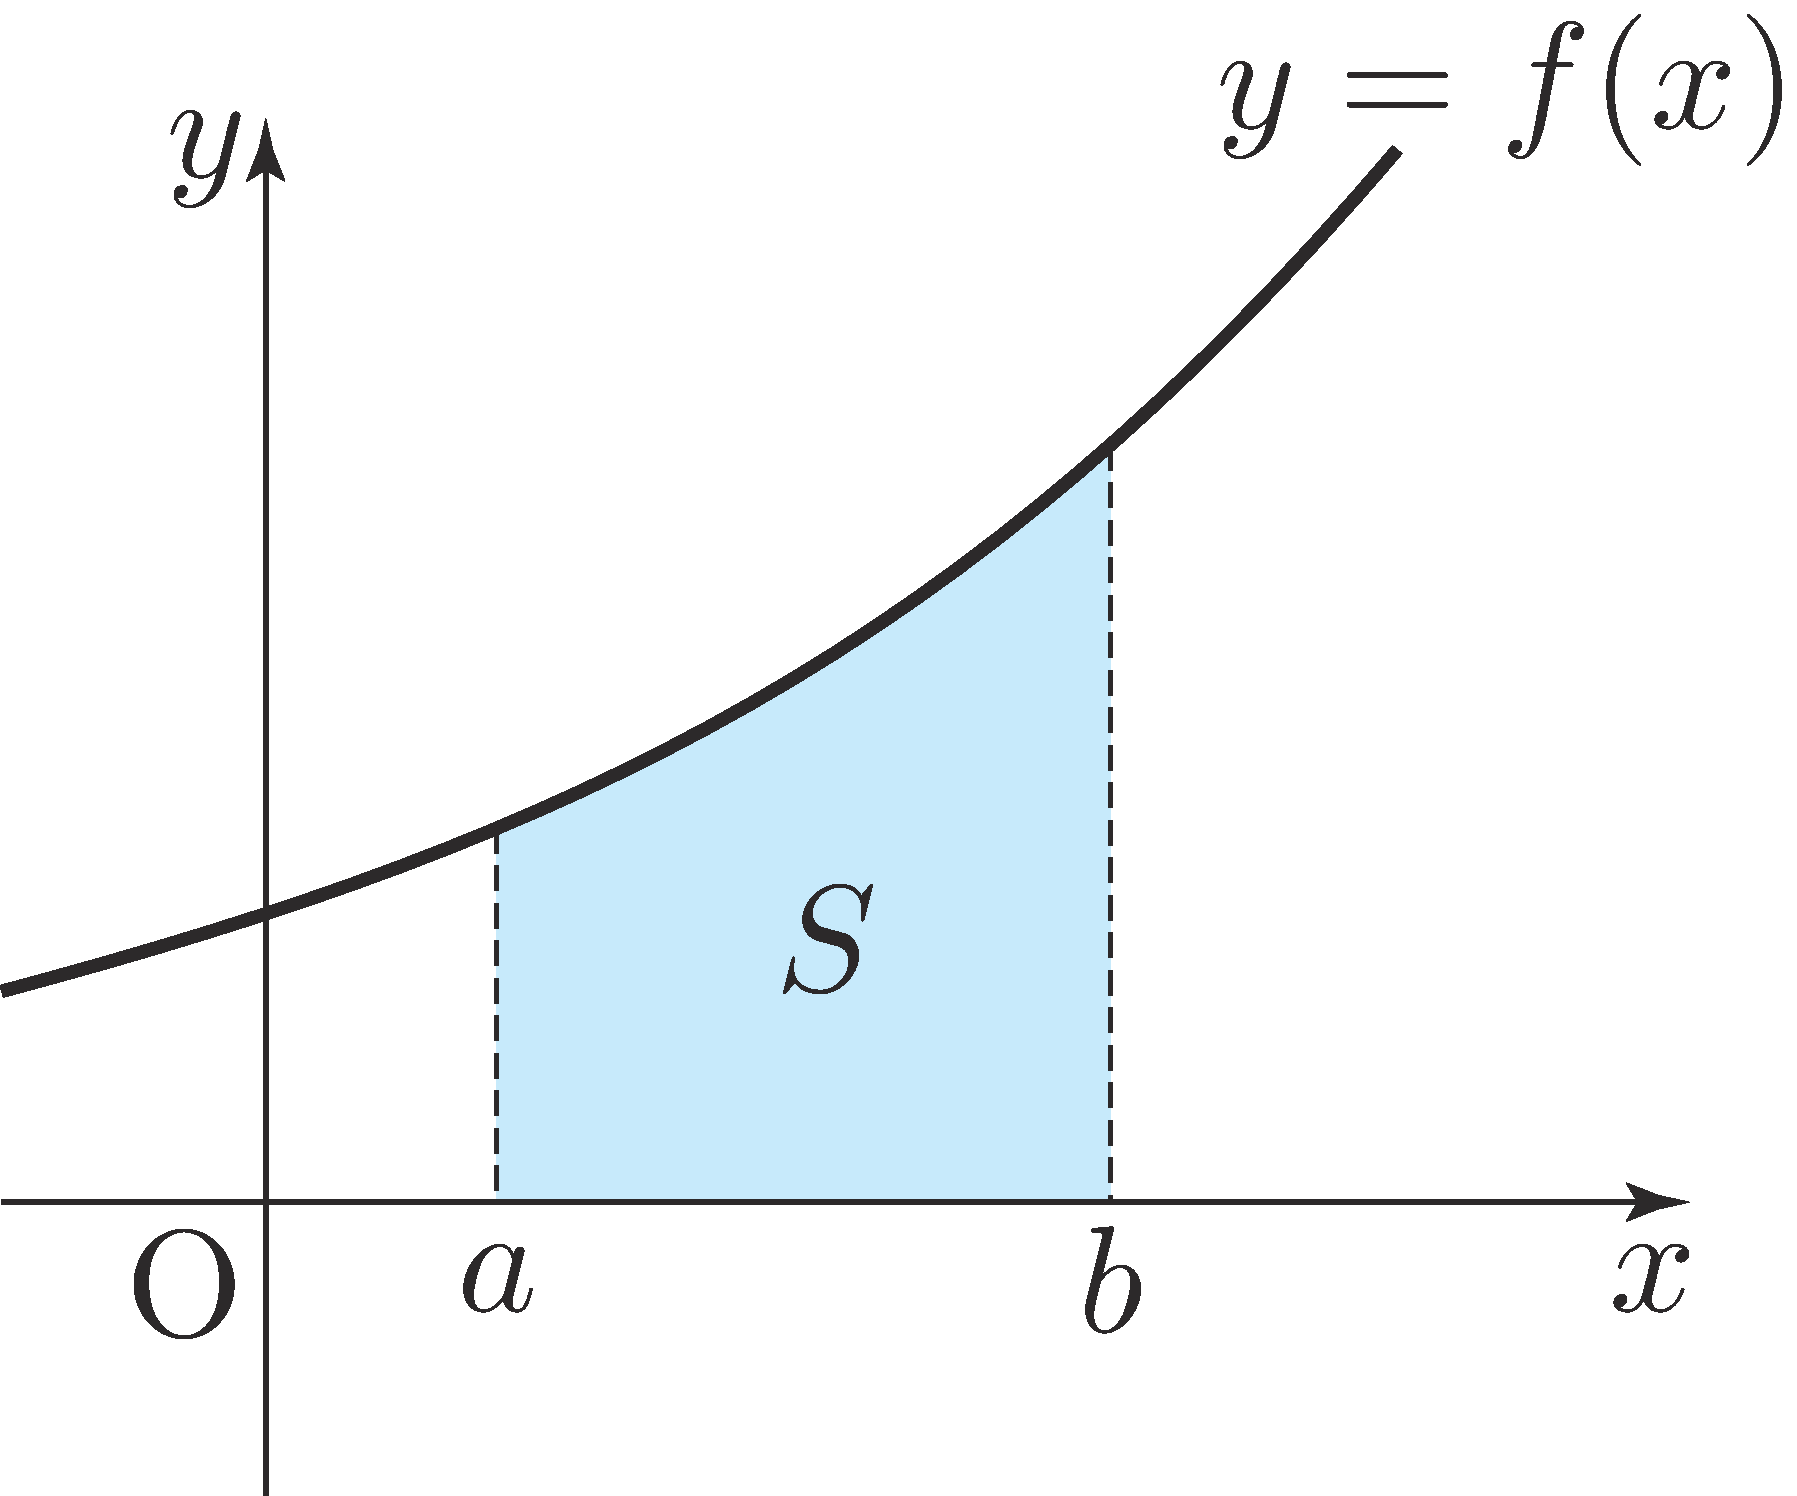
\includegraphics[scale=\pgfkeysvalueof{picsize}]{DBs/pic/zerr_11_1.pdf}}\
\qquad
\centering \subfloat[][]{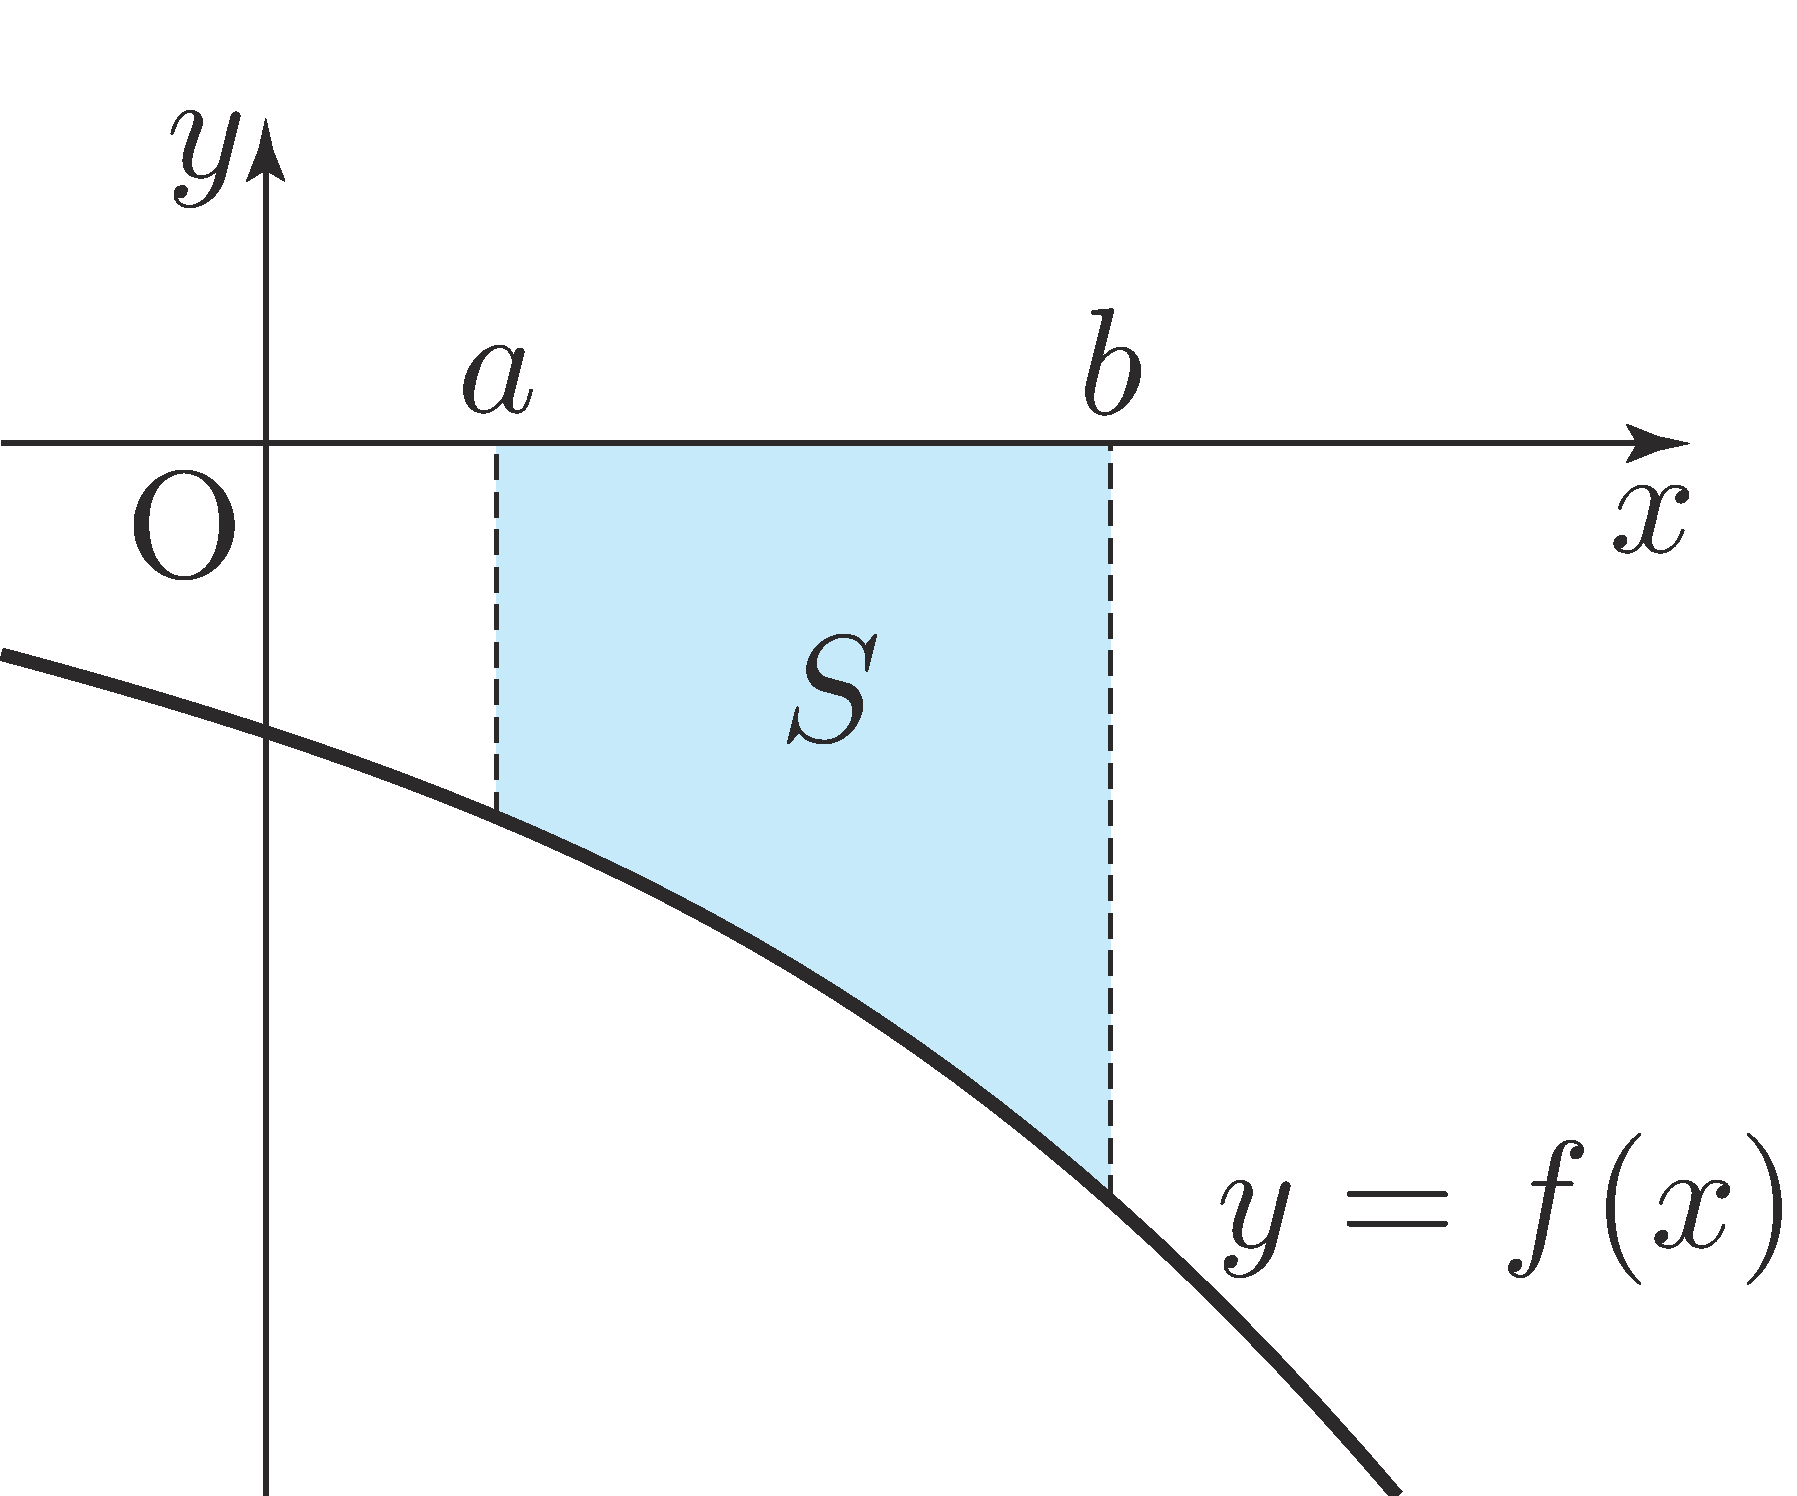
\includegraphics[scale=\pgfkeysvalueof{picsize}]{DBs/pic/zerr_11_2.pdf}}\
\end{figure}


$\CCI ab$에서 함수 $y=f\left( x \right) $의 구간넓이를 $S$라 하겠습니다. (a)와 같이 $f\left( x \right)\ge 0$이면 $S= \int_{a}^{b}f\left( x \right) dx$입니다. (b)와 같이 $f\left( x \right)\le0 $이면  $S=\int_{a}^{b}\left\{ -f\left( x \right) \right\} dx $입니다. 이를 종합하면 $f\left( x \right) $의 부호와 관계없이 $S=\int_{a}^{b}\abs{f\left( x \right) }dx$입니다. 

\begin{center}
    \centering 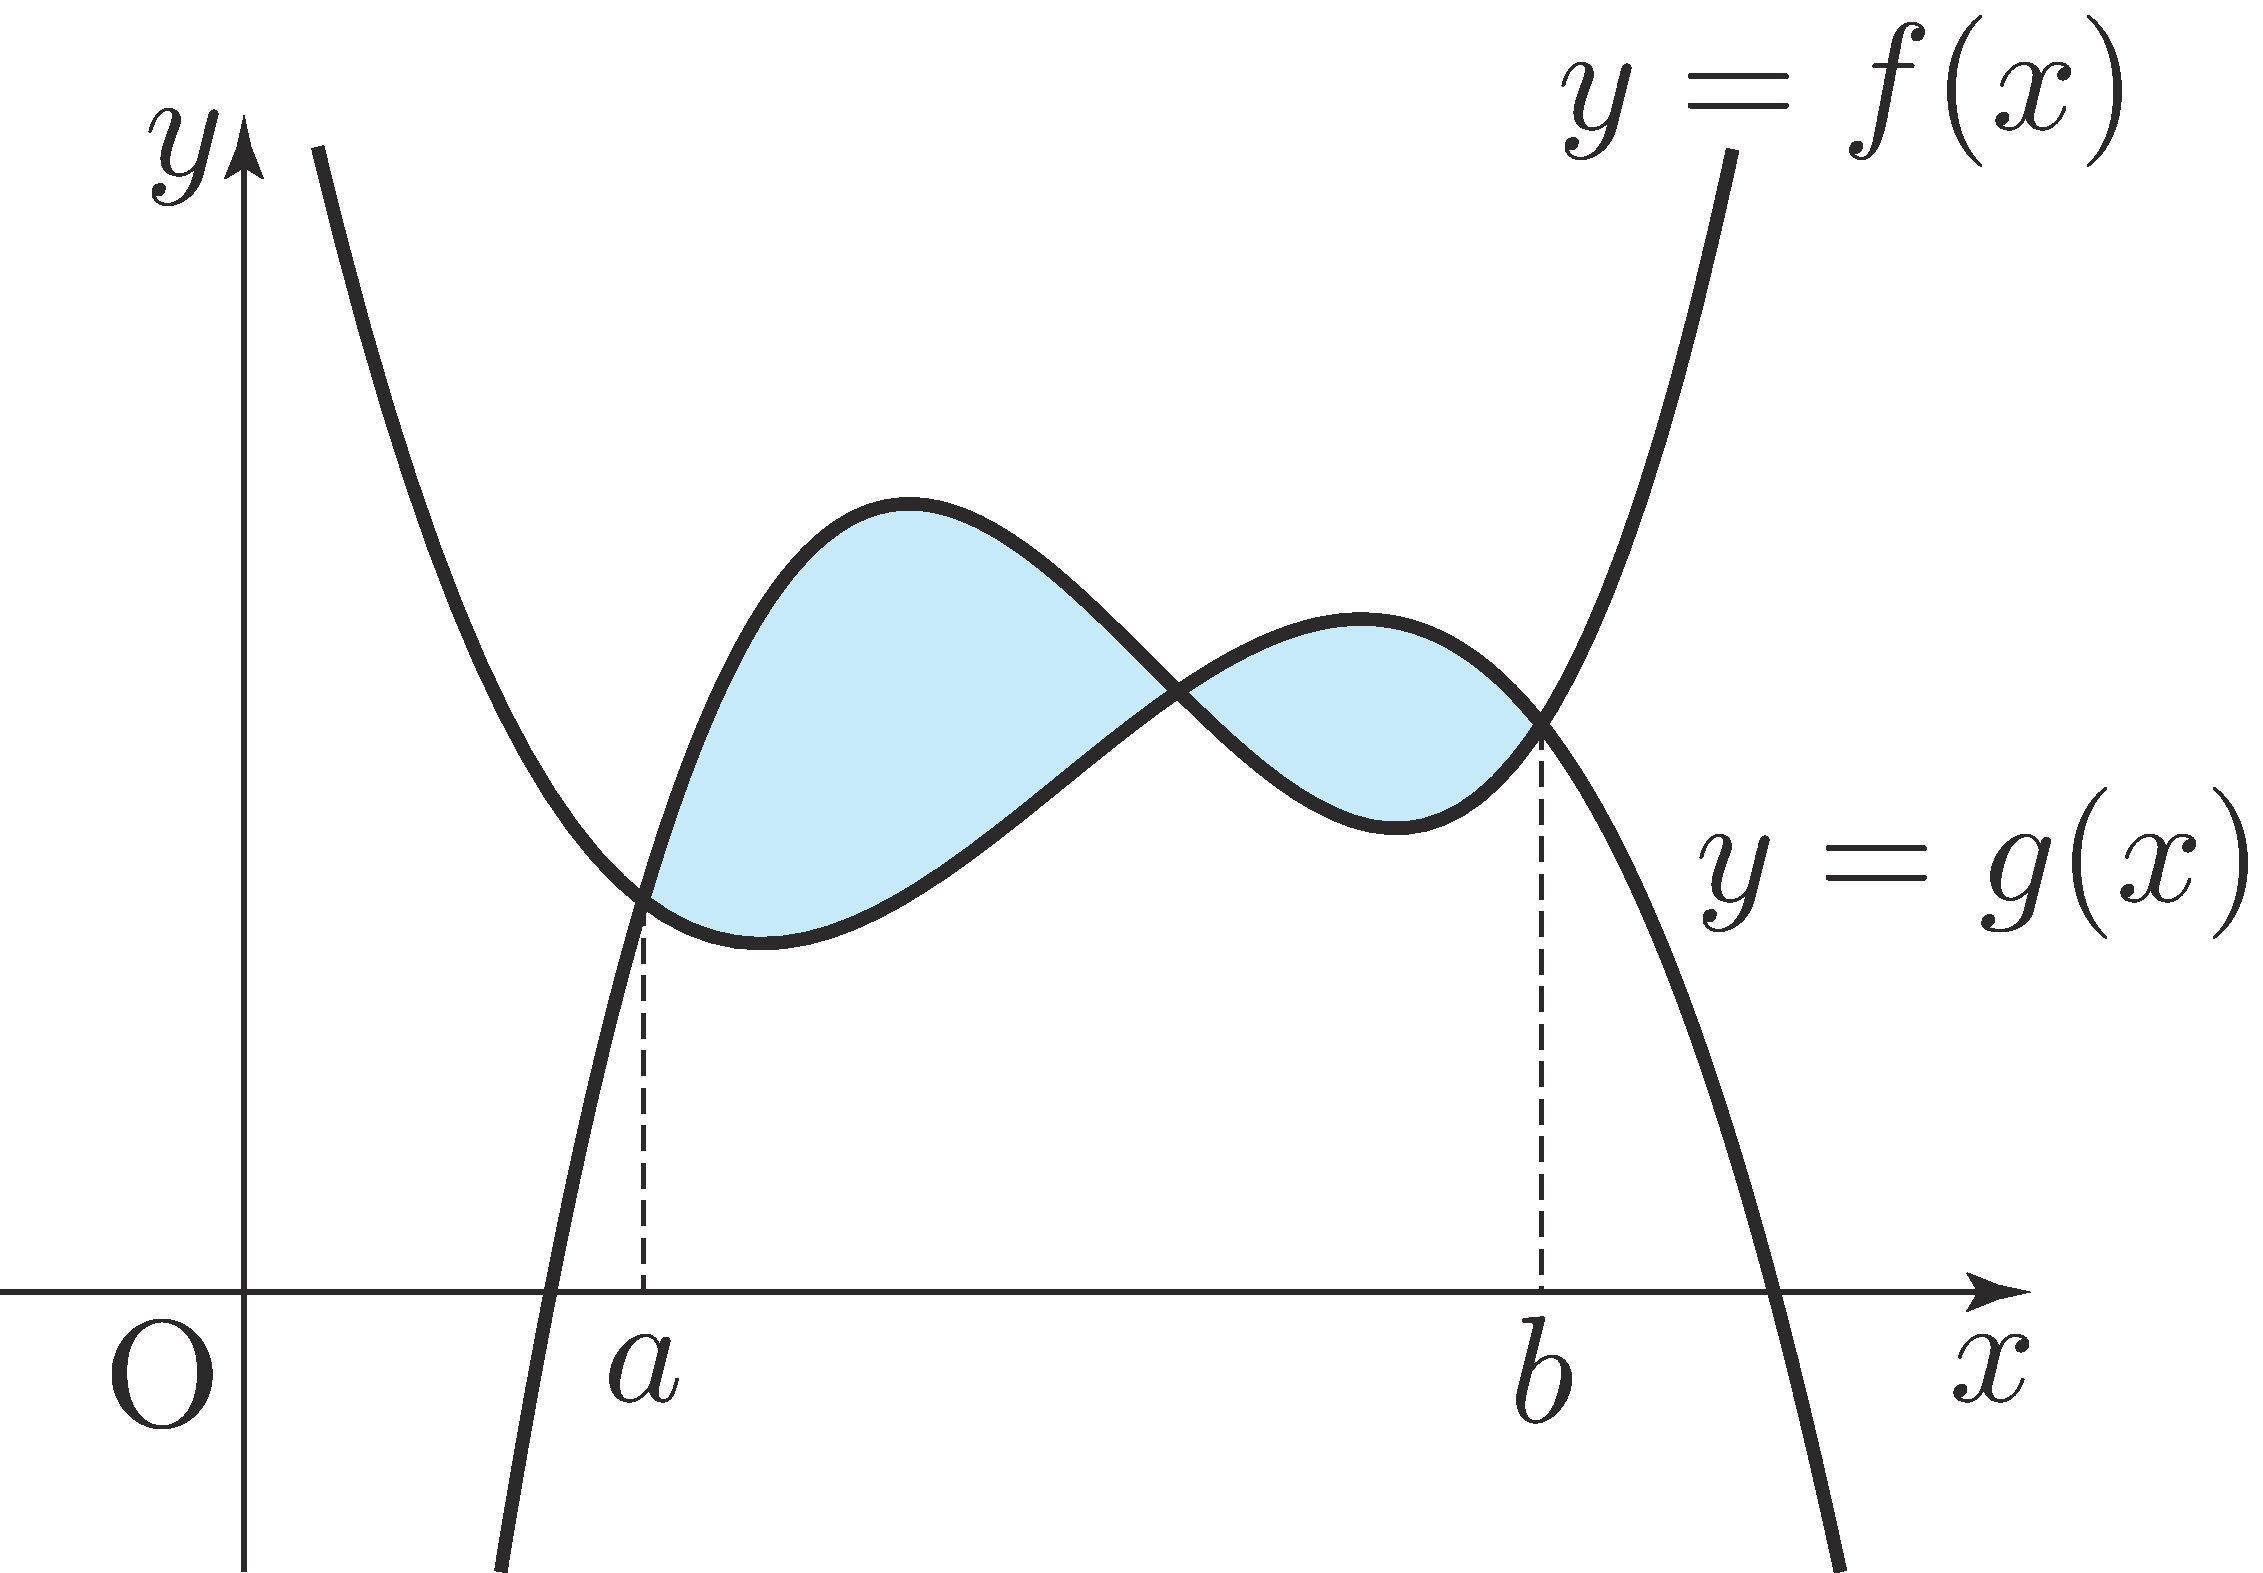
\includegraphics[scale=\pgfkeysvalueof{picsize}]{DBs/pic/zerr_13.pdf}\
    \end{center}    
    $\CCI ab$에서 두 함수 $y=f\left( x \right) $, $y=g\left( x \right) $와 두 직선 $x=a$, $x=b$로 둘러싸인 부분의 넓이는 $\int_{a}^{b}\abs{f\left( x \right)-g\left( x \right)  }dx$입니다.


\subsection{물리학(속력, 속도, 거리)}
미분과 마찬가지로 적분으로 물리학의 개념을 설명할 수 있습니다. 자세한 내용은 Calc에서 다룹니다.

\clearpage














